% Options for packages loaded elsewhere
\PassOptionsToPackage{unicode}{hyperref}
\PassOptionsToPackage{hyphens}{url}
%
\documentclass[
]{book}
\usepackage{amsmath,amssymb}
\usepackage{lmodern}
\usepackage{iftex}
\ifPDFTeX
  \usepackage[T1]{fontenc}
  \usepackage[utf8]{inputenc}
  \usepackage{textcomp} % provide euro and other symbols
\else % if luatex or xetex
  \usepackage{unicode-math}
  \defaultfontfeatures{Scale=MatchLowercase}
  \defaultfontfeatures[\rmfamily]{Ligatures=TeX,Scale=1}
\fi
% Use upquote if available, for straight quotes in verbatim environments
\IfFileExists{upquote.sty}{\usepackage{upquote}}{}
\IfFileExists{microtype.sty}{% use microtype if available
  \usepackage[]{microtype}
  \UseMicrotypeSet[protrusion]{basicmath} % disable protrusion for tt fonts
}{}
\makeatletter
\@ifundefined{KOMAClassName}{% if non-KOMA class
  \IfFileExists{parskip.sty}{%
    \usepackage{parskip}
  }{% else
    \setlength{\parindent}{0pt}
    \setlength{\parskip}{6pt plus 2pt minus 1pt}}
}{% if KOMA class
  \KOMAoptions{parskip=half}}
\makeatother
\usepackage{xcolor}
\IfFileExists{xurl.sty}{\usepackage{xurl}}{} % add URL line breaks if available
\IfFileExists{bookmark.sty}{\usepackage{bookmark}}{\usepackage{hyperref}}
\hypersetup{
  pdftitle={Graph Algorithms},
  pdfauthor={CS 225 Course Staff},
  hidelinks,
  pdfcreator={LaTeX via pandoc}}
\urlstyle{same} % disable monospaced font for URLs
\usepackage{color}
\usepackage{fancyvrb}
\newcommand{\VerbBar}{|}
\newcommand{\VERB}{\Verb[commandchars=\\\{\}]}
\DefineVerbatimEnvironment{Highlighting}{Verbatim}{commandchars=\\\{\}}
% Add ',fontsize=\small' for more characters per line
\usepackage{framed}
\definecolor{shadecolor}{RGB}{248,248,248}
\newenvironment{Shaded}{\begin{snugshade}}{\end{snugshade}}
\newcommand{\AlertTok}[1]{\textcolor[rgb]{0.94,0.16,0.16}{#1}}
\newcommand{\AnnotationTok}[1]{\textcolor[rgb]{0.56,0.35,0.01}{\textbf{\textit{#1}}}}
\newcommand{\AttributeTok}[1]{\textcolor[rgb]{0.77,0.63,0.00}{#1}}
\newcommand{\BaseNTok}[1]{\textcolor[rgb]{0.00,0.00,0.81}{#1}}
\newcommand{\BuiltInTok}[1]{#1}
\newcommand{\CharTok}[1]{\textcolor[rgb]{0.31,0.60,0.02}{#1}}
\newcommand{\CommentTok}[1]{\textcolor[rgb]{0.56,0.35,0.01}{\textit{#1}}}
\newcommand{\CommentVarTok}[1]{\textcolor[rgb]{0.56,0.35,0.01}{\textbf{\textit{#1}}}}
\newcommand{\ConstantTok}[1]{\textcolor[rgb]{0.00,0.00,0.00}{#1}}
\newcommand{\ControlFlowTok}[1]{\textcolor[rgb]{0.13,0.29,0.53}{\textbf{#1}}}
\newcommand{\DataTypeTok}[1]{\textcolor[rgb]{0.13,0.29,0.53}{#1}}
\newcommand{\DecValTok}[1]{\textcolor[rgb]{0.00,0.00,0.81}{#1}}
\newcommand{\DocumentationTok}[1]{\textcolor[rgb]{0.56,0.35,0.01}{\textbf{\textit{#1}}}}
\newcommand{\ErrorTok}[1]{\textcolor[rgb]{0.64,0.00,0.00}{\textbf{#1}}}
\newcommand{\ExtensionTok}[1]{#1}
\newcommand{\FloatTok}[1]{\textcolor[rgb]{0.00,0.00,0.81}{#1}}
\newcommand{\FunctionTok}[1]{\textcolor[rgb]{0.00,0.00,0.00}{#1}}
\newcommand{\ImportTok}[1]{#1}
\newcommand{\InformationTok}[1]{\textcolor[rgb]{0.56,0.35,0.01}{\textbf{\textit{#1}}}}
\newcommand{\KeywordTok}[1]{\textcolor[rgb]{0.13,0.29,0.53}{\textbf{#1}}}
\newcommand{\NormalTok}[1]{#1}
\newcommand{\OperatorTok}[1]{\textcolor[rgb]{0.81,0.36,0.00}{\textbf{#1}}}
\newcommand{\OtherTok}[1]{\textcolor[rgb]{0.56,0.35,0.01}{#1}}
\newcommand{\PreprocessorTok}[1]{\textcolor[rgb]{0.56,0.35,0.01}{\textit{#1}}}
\newcommand{\RegionMarkerTok}[1]{#1}
\newcommand{\SpecialCharTok}[1]{\textcolor[rgb]{0.00,0.00,0.00}{#1}}
\newcommand{\SpecialStringTok}[1]{\textcolor[rgb]{0.31,0.60,0.02}{#1}}
\newcommand{\StringTok}[1]{\textcolor[rgb]{0.31,0.60,0.02}{#1}}
\newcommand{\VariableTok}[1]{\textcolor[rgb]{0.00,0.00,0.00}{#1}}
\newcommand{\VerbatimStringTok}[1]{\textcolor[rgb]{0.31,0.60,0.02}{#1}}
\newcommand{\WarningTok}[1]{\textcolor[rgb]{0.56,0.35,0.01}{\textbf{\textit{#1}}}}
\usepackage{longtable,booktabs,array}
\usepackage{calc} % for calculating minipage widths
% Correct order of tables after \paragraph or \subparagraph
\usepackage{etoolbox}
\makeatletter
\patchcmd\longtable{\par}{\if@noskipsec\mbox{}\fi\par}{}{}
\makeatother
% Allow footnotes in longtable head/foot
\IfFileExists{footnotehyper.sty}{\usepackage{footnotehyper}}{\usepackage{footnote}}
\makesavenoteenv{longtable}
\usepackage{graphicx}
\makeatletter
\def\maxwidth{\ifdim\Gin@nat@width>\linewidth\linewidth\else\Gin@nat@width\fi}
\def\maxheight{\ifdim\Gin@nat@height>\textheight\textheight\else\Gin@nat@height\fi}
\makeatother
% Scale images if necessary, so that they will not overflow the page
% margins by default, and it is still possible to overwrite the defaults
% using explicit options in \includegraphics[width, height, ...]{}
\setkeys{Gin}{width=\maxwidth,height=\maxheight,keepaspectratio}
% Set default figure placement to htbp
\makeatletter
\def\fps@figure{htbp}
\makeatother
\setlength{\emergencystretch}{3em} % prevent overfull lines
\providecommand{\tightlist}{%
  \setlength{\itemsep}{0pt}\setlength{\parskip}{0pt}}
\setcounter{secnumdepth}{5}
\ifLuaTeX
  \usepackage{selnolig}  % disable illegal ligatures
\fi
\usepackage[]{natbib}
\bibliographystyle{plainnat}

\title{Graph Algorithms}
\author{CS 225 Course Staff}
\date{2022-10-26}

\begin{document}
\maketitle

{
\setcounter{tocdepth}{2}
\tableofcontents
}
\hypertarget{data-structures-in-c}{%
\chapter{Data Structures in C++}\label{data-structures-in-c}}

\emph{hugs}

Welcome to the Course Staff produced coursebook to pair with CS 225! We hope this really helps you learn more and improves your code. Report any issues at our Github repo and we'll be sure to credit you as well :)

\hypertarget{c-introduction}{%
\chapter{C++ Introduction}\label{c-introduction}}

\hypertarget{arrays-and-lists}{%
\chapter{Arrays and Lists}\label{arrays-and-lists}}

\hypertarget{trees}{%
\chapter{Trees}\label{trees}}

Trees are a hierarchical data structure with a certain set of properties that distinguish it from graphs. Trees are rooted, which means that there is a pointer to the root node and each child node can be reached via the root.

\hypertarget{basic-tree-terminology}{%
\section{Basic tree terminology}\label{basic-tree-terminology}}

(adapted from CS 173)
* Vertex: ``nodes''

\begin{itemize}
\item
  Path: sequence of edges
\item
  Parents: Node \textbf{b, d, x} have Node \textbf{a} as their parent
\item
  Children: \textbf{b, d, x,} are the children of \textbf{a}
\item
  Siblings: \textbf{b, d, x,} are siblings of each other
\item
  Ancestors: \textbf{u} has ancestors \textbf{l, d, a}
\item
  Descendants: \textbf{x} has \textbf{s, m} as its descendants
\item
  Leaves: Vertices with no children
\end{itemize}

\hypertarget{tree-property-height}{%
\section{Tree Property: Height}\label{tree-property-height}}

\begin{itemize}
\tightlist
\item
  \textbf{Computation of the tree height}

  \begin{itemize}
  \tightlist
  \item
    The length of the longest path from the root to the leaf (count edges).
  \item
    If we want to compute recursively:
  \end{itemize}

  height(T) = 1 + max(height(TL), height(TR)), where if height(null) = -1, which might be counter-intuitive but it follows the mathematical definition of tree height
\end{itemize}

\hypertarget{tree-property-binary}{%
\section{Tree Property: Binary}\label{tree-property-binary}}

\begin{itemize}
\tightlist
\item
  A binary tree is either

  \begin{itemize}
  \tightlist
  \item
    T = \{TL, TR, r\}, where TL, TR are binary trees
  \item
    T = \{\} = ~\(\emptyset\)
  \end{itemize}
\end{itemize}

\hypertarget{tree-property-full}{%
\section{Tree Property: Full}\label{tree-property-full}}

\begin{itemize}
\tightlist
\item
  A binary tree is full \emph{if and only if}

  \begin{itemize}
  \tightlist
  \item
    Either: F = \{\}
  \item
    Or: F = \{TL, TR, r\} where TL, TR both have either 0 or 2 children
  \end{itemize}
\item
  \textbf{Theorem}: A binary tree with n data items has n+1 null pointers.
\end{itemize}

\hypertarget{tree-property-perfect}{%
\section{Tree Property: Perfect}\label{tree-property-perfect}}

\begin{itemize}
\tightlist
\item
  A perfect tree Ph is defined by its height

  \begin{itemize}
  \tightlist
  \item
    Ph is a tree of height \textbf{h}, with

    \begin{itemize}
    \tightlist
    \item
      P-1 = \{\}
    \item
      Ph = \{r, Ph-1, Ph-1\} when h\textgreater=0
    \end{itemize}
  \end{itemize}
\end{itemize}

\hypertarget{tree-property-complete}{%
\section{Tree Property: Complete}\label{tree-property-complete}}

(as defined in data structures)
* A complete tree is
* A perfect tree except for the last level

\begin{itemize}
\item
  All leaves must be pushed to the \textbf{left}
\item
  Or, recursively, a complete tree \textbf{Ch} of height \textbf{h} is

  \begin{itemize}
  \item
    C-1 = \{\}
  \item
    Ch = \{r, TL, TR\} where

    \begin{itemize}
    \tightlist
    \item
      Either: TL = Ch-1 and TR = Ph-2
      Or:TL = Ph-1 and TR = Ch-1
    \end{itemize}
  \end{itemize}
\end{itemize}

\begin{itemize}
\tightlist
\item
  Full does not imply perfect, so as complete does not imply perfect
\item
  Not full implies not perfect, thus perfect implies full; perfect also implies complete too.
\end{itemize}

\hypertarget{tree-traversals}{%
\section{Tree Traversals}\label{tree-traversals}}

(practice them here: \url{https://yongdanielliang.github.io/animation/web/BST.html})
* Pre-Order: process the data first, then left child, then the right child
* In-Order: left child, process the data, right child
* Post-Order: left child, right child, process the data last

\begin{Shaded}
\begin{Highlighting}[]
\DataTypeTok{void}\NormalTok{ BinaryTree}\OperatorTok{\textless{}}\NormalTok{T}\OperatorTok{\textgreater{}::}\NormalTok{preOrder}\OperatorTok{(}\NormalTok{TreeNode }\OperatorTok{*}\NormalTok{ cur}\OperatorTok{)} \OperatorTok{\{}
    \ControlFlowTok{if} \OperatorTok{(}\NormalTok{cur }\OperatorTok{!=}\NormalTok{ NULL}\OperatorTok{)} \OperatorTok{\{}
\NormalTok{        func}\OperatorTok{(}\NormalTok{curr}\OperatorTok{{-}\textgreater{}}\NormalTok{data}\OperatorTok{);}
\NormalTok{        preOrder}\OperatorTok{(}\NormalTok{curr}\OperatorTok{{-}\textgreater{}}\NormalTok{left}\OperatorTok{);}
\NormalTok{        preOrder}\OperatorTok{(}\NormalTok{curr}\OperatorTok{{-}\textgreater{}}\NormalTok{right}\OperatorTok{);}
    \OperatorTok{\}}
\OperatorTok{\}}

\DataTypeTok{void}\NormalTok{ BinaryTree}\OperatorTok{\textless{}}\NormalTok{T}\OperatorTok{\textgreater{}::}\NormalTok{inOrder}\OperatorTok{(}\NormalTok{TreeNode }\OperatorTok{*}\NormalTok{ cur}\OperatorTok{)} \OperatorTok{\{}
    \ControlFlowTok{if} \OperatorTok{(}\NormalTok{cur }\OperatorTok{!=}\NormalTok{ NULL}\OperatorTok{)} \OperatorTok{\{}
\NormalTok{        preOrder}\OperatorTok{(}\NormalTok{curr}\OperatorTok{{-}\textgreater{}}\NormalTok{left}\OperatorTok{);}
\NormalTok{        func}\OperatorTok{(}\NormalTok{curr}\OperatorTok{{-}\textgreater{}}\NormalTok{data}\OperatorTok{);}
\NormalTok{        preOrder}\OperatorTok{(}\NormalTok{curr}\OperatorTok{{-}\textgreater{}}\NormalTok{right}\OperatorTok{);}
    \OperatorTok{\}}
\OperatorTok{\}}

\DataTypeTok{void}\NormalTok{ BinaryTree}\OperatorTok{\textless{}}\NormalTok{T}\OperatorTok{\textgreater{}::}\NormalTok{inOrder}\OperatorTok{(}\NormalTok{TreeNode }\OperatorTok{*}\NormalTok{ cur}\OperatorTok{)} \OperatorTok{\{}
    \ControlFlowTok{if} \OperatorTok{(}\NormalTok{cur }\OperatorTok{!=}\NormalTok{ NULL}\OperatorTok{)} \OperatorTok{\{}
\NormalTok{        preOrder}\OperatorTok{(}\NormalTok{curr}\OperatorTok{{-}\textgreater{}}\NormalTok{left}\OperatorTok{);}
\NormalTok{        preOrder}\OperatorTok{(}\NormalTok{curr}\OperatorTok{{-}\textgreater{}}\NormalTok{right}\OperatorTok{);}
\NormalTok{        func}\OperatorTok{(}\NormalTok{curr}\OperatorTok{{-}\textgreater{}}\NormalTok{data}\OperatorTok{);}
    \OperatorTok{\}}
\OperatorTok{\}}
\end{Highlighting}
\end{Shaded}

\hypertarget{searching-trees}{%
\section{Searching Trees}\label{searching-trees}}

\begin{itemize}
\item
  BFS: breadth first search: visits nodes at each level (level-order traversal): use a queue
\item
  DFS: depth first search: find the endpoint of the path quickly (in order, pre order or post order): use a stack
\item
  Traversal vs Search: traverse visits every node vs search visits nodes until you find what you want
\end{itemize}

\hypertarget{delete-and-insert}{%
\section{Delete and Insert}\label{delete-and-insert}}

\hypertarget{binary-search-trees}{%
\chapter{Binary Search Trees}\label{binary-search-trees}}

\hypertarget{avl-trees}{%
\chapter{AVL Trees}\label{avl-trees}}

\hypertarget{heaps}{%
\chapter{Heaps}\label{heaps}}

\begin{figure}
\centering
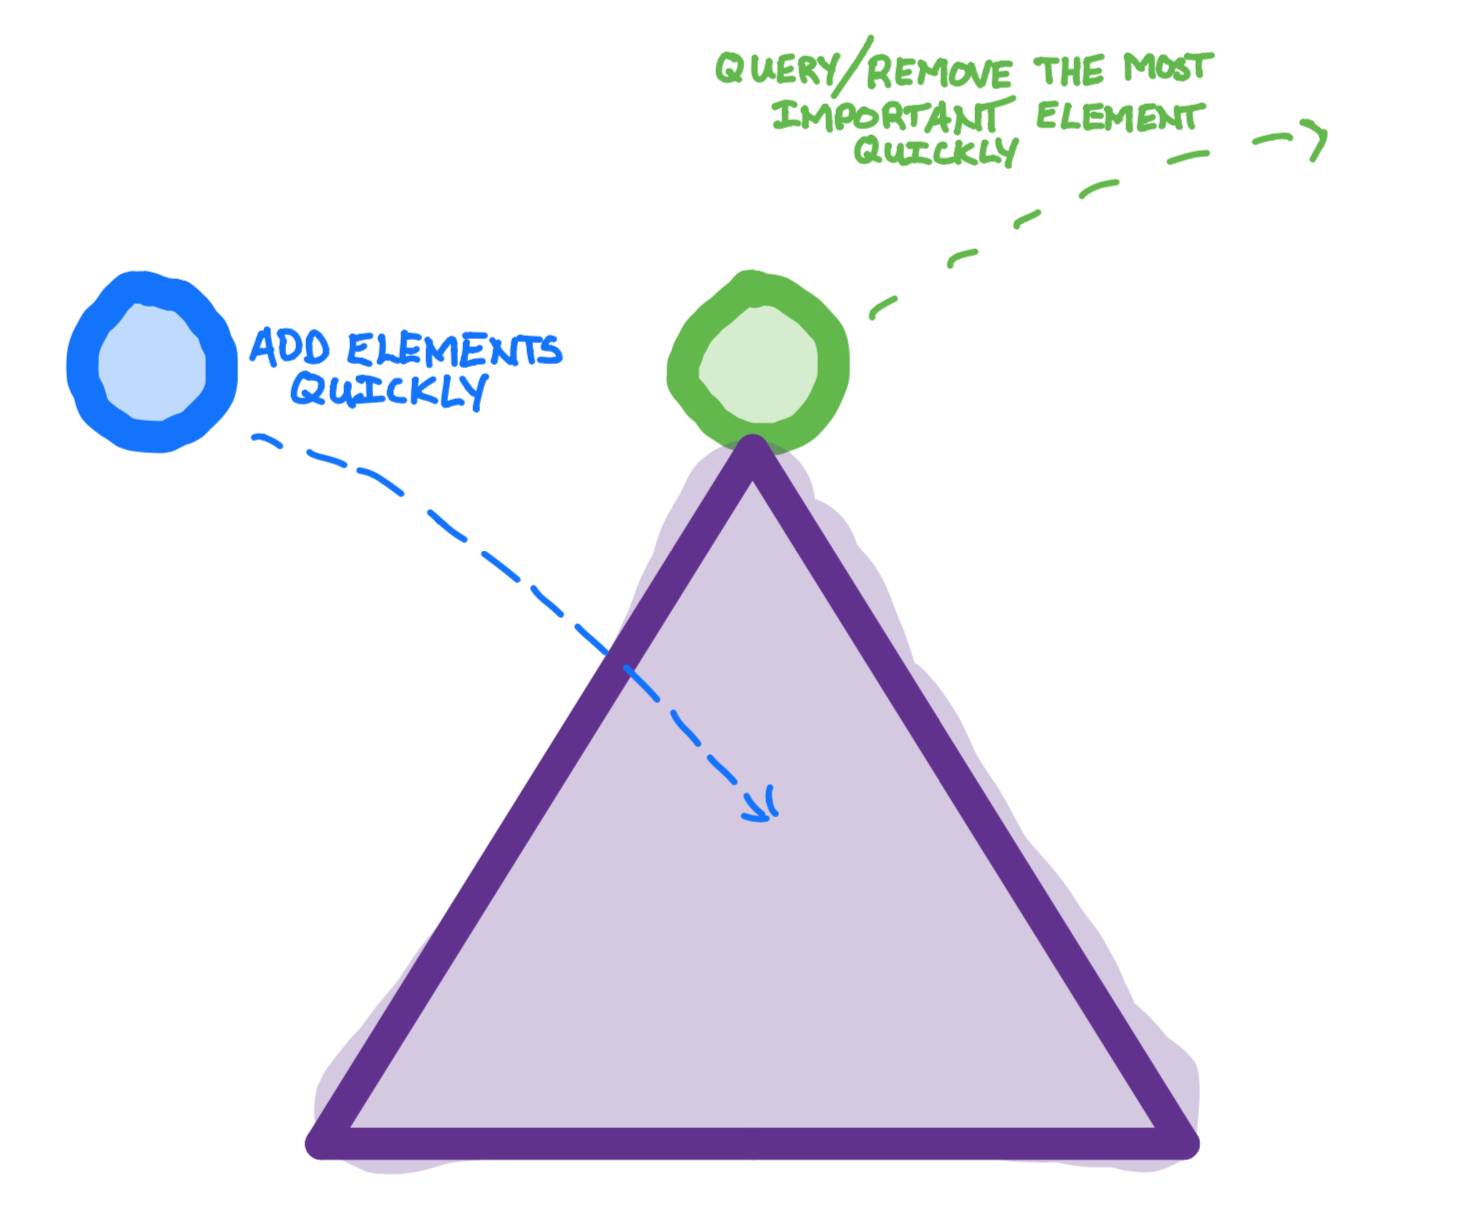
\includegraphics{images/heaps/heap.png}
\caption{Heaps - Add elements quickly and query/remove the most important element quickly}
\end{figure}

\hypertarget{uses}{%
\section{Uses}\label{uses}}

\begin{itemize}
\item
  getting the smallest/largest item each time in succession
\item
  maintaining top or bottom k elements, getting the median of large datasets
\item
  sorting data via heap sort
\end{itemize}

\hypertarget{pre-reqs-of-the-data}{%
\subsection{Pre reqs of the data}\label{pre-reqs-of-the-data}}

\begin{itemize}
\item
  Has to be orderable
\item
  Has to have \texttt{\textgreater{}} implemented
\end{itemize}

\hypertarget{adt-implementation-functions}{%
\subsection{ADT implementation functions}\label{adt-implementation-functions}}

\begin{itemize}
\tightlist
\item
  insert
\item
  remove
\item
  isEmpty
\end{itemize}

\hypertarget{min-heap-vs-max-heap}{%
\section{min heap vs max heap}\label{min-heap-vs-max-heap}}

\begin{itemize}
\item
  min heap is smallest at top and higher at the bottom
\item
  max heap is the largest at top and goes smaller at the bottom
\item
  the logic is basically the same in either case, just inverted - we'll do min heap here but the similar prinicples apply to max heap quite easily
\end{itemize}

\hypertarget{array-based-implementation}{%
\section{Array based implementation}\label{array-based-implementation}}

\begin{itemize}
\item
  the simplest way to do it is with arrays that has each level contiguous
\item
  it makes swaps and indexing easy
\item
  not having to deal with pointers as much - we're used to arrays
\end{itemize}

\hypertarget{compare-to-other-implementations}{%
\subsection{Compare to other implementations}\label{compare-to-other-implementations}}

\begin{itemize}
\tightlist
\item
  unsorted
\end{itemize}

\hypertarget{insert---heapify-up}{%
\section{insert() - Heapify up}\label{insert---heapify-up}}

\begin{itemize}
\tightlist
\item
  Add a bottom
\end{itemize}

\hypertarget{heapify-down}{%
\section{Heapify down}\label{heapify-down}}

\hypertarget{build-heap}{%
\section{Build heap}\label{build-heap}}

\begin{figure}
\centering
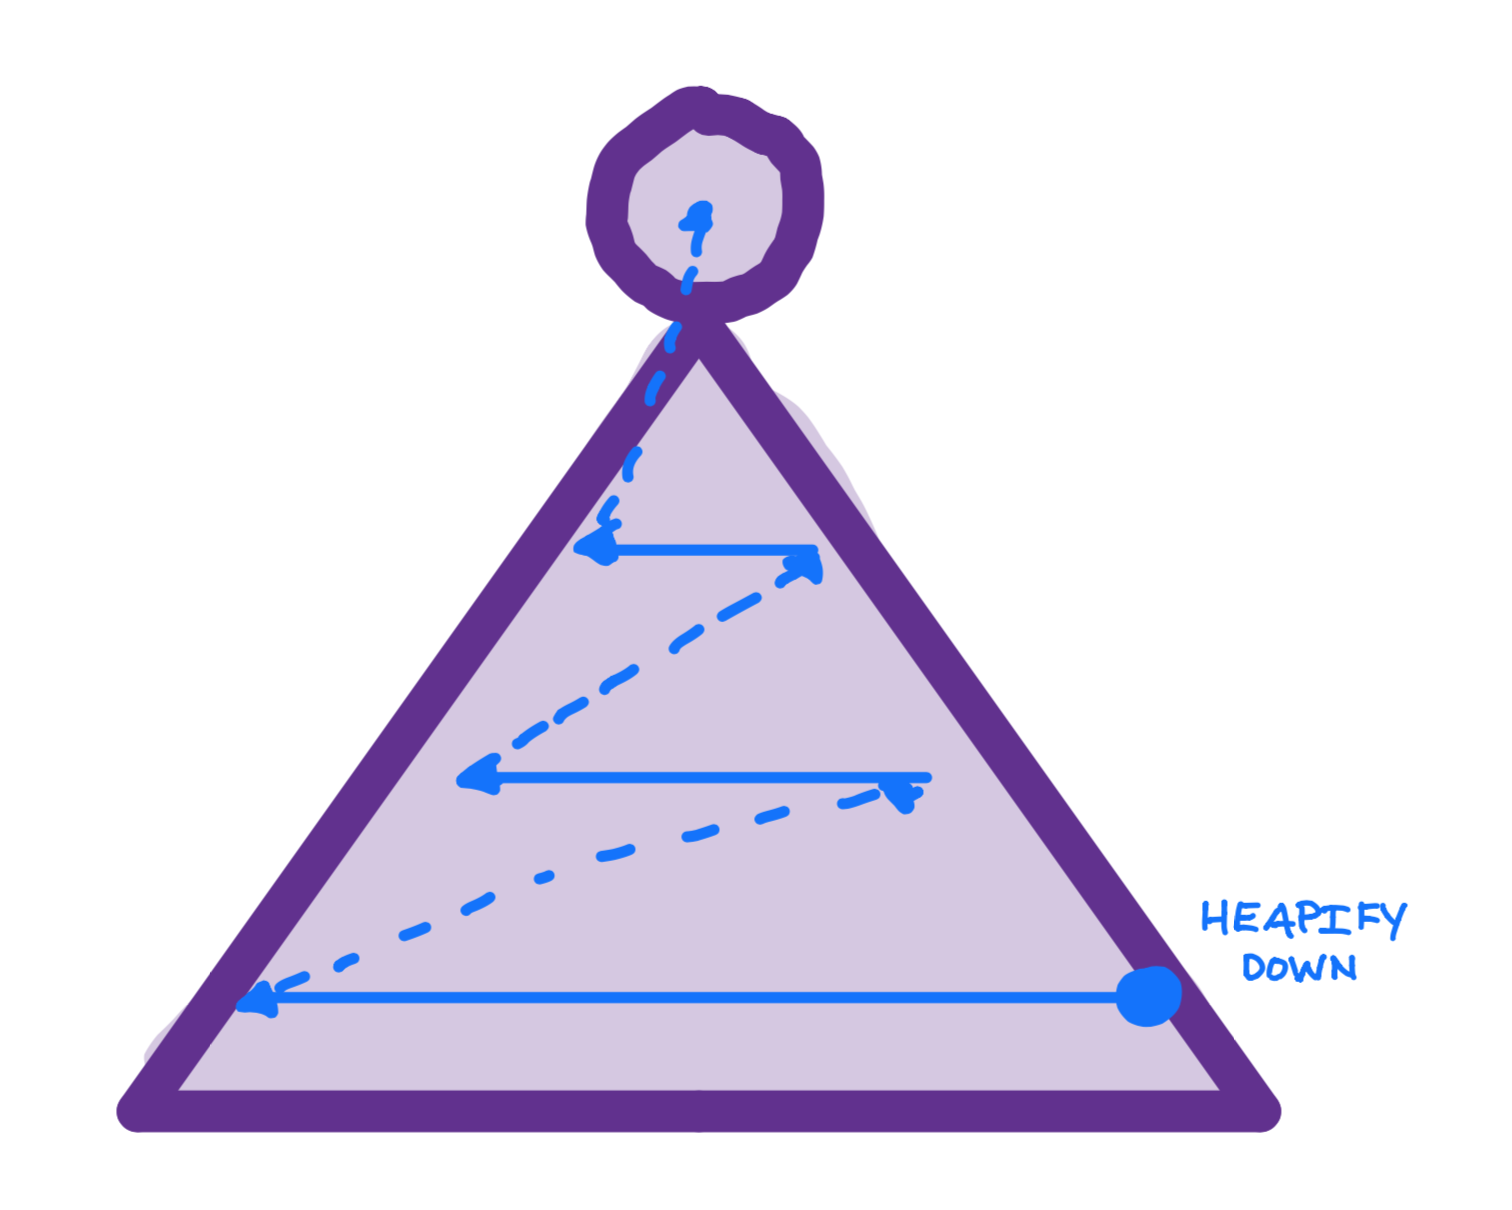
\includegraphics{images/heaps/build_heap.png}
\caption{To build a Heap in linear time we heapify down from the bottom to the top}
\end{figure}

\hypertarget{recursive-proof}{%
\subsection{Recursive proof}\label{recursive-proof}}

\hypertarget{heap-sort}{%
\section{Heap Sort}\label{heap-sort}}

\hypertarget{priority-queue}{%
\section{Priority Queue}\label{priority-queue}}

\hypertarget{see-also}{%
\section{See also:}\label{see-also}}

\begin{itemize}
\item
  \href{https://medium.com/basecs/learning-to-love-heaps-cef2b273a238}{Learning to Love Heaps} Long Medium Post by Vaidehi Joshi
\item
  \href{https://www.youtube.com/watch?v=c1TpLRyQJ4w}{Introduction to a Heap} Video Series by Paul Programming
\item
  \href{https://courses.engr.illinois.edu/cs225/sp2021/resources/heaps/}{Old CS 225 resources page} by Eddie Huang
\end{itemize}

\hypertarget{disjoint-sets}{%
\chapter{Disjoint Sets}\label{disjoint-sets}}

\hypertarget{b-trees}{%
\chapter{B Trees}\label{b-trees}}

\hypertarget{hashing}{%
\chapter{Hashing}\label{hashing}}

\hypertarget{graphs}{%
\chapter{Graphs}\label{graphs}}

\hypertarget{graph-algorithms}{%
\chapter{Graph Algorithms}\label{graph-algorithms}}

\end{document}
